\section{Séquence de potentiel d’action (spike train)}
Les mécanorécepteurs produisent une séquence de potentiel d’action dont l’amplitude et la fréquence est propre à la caractéristique de la sensation. La séquence de potentiel d’action peut alors être interprété comme l’encodage de la sensation.\par
\begin{figure}[!h]
	\centering
	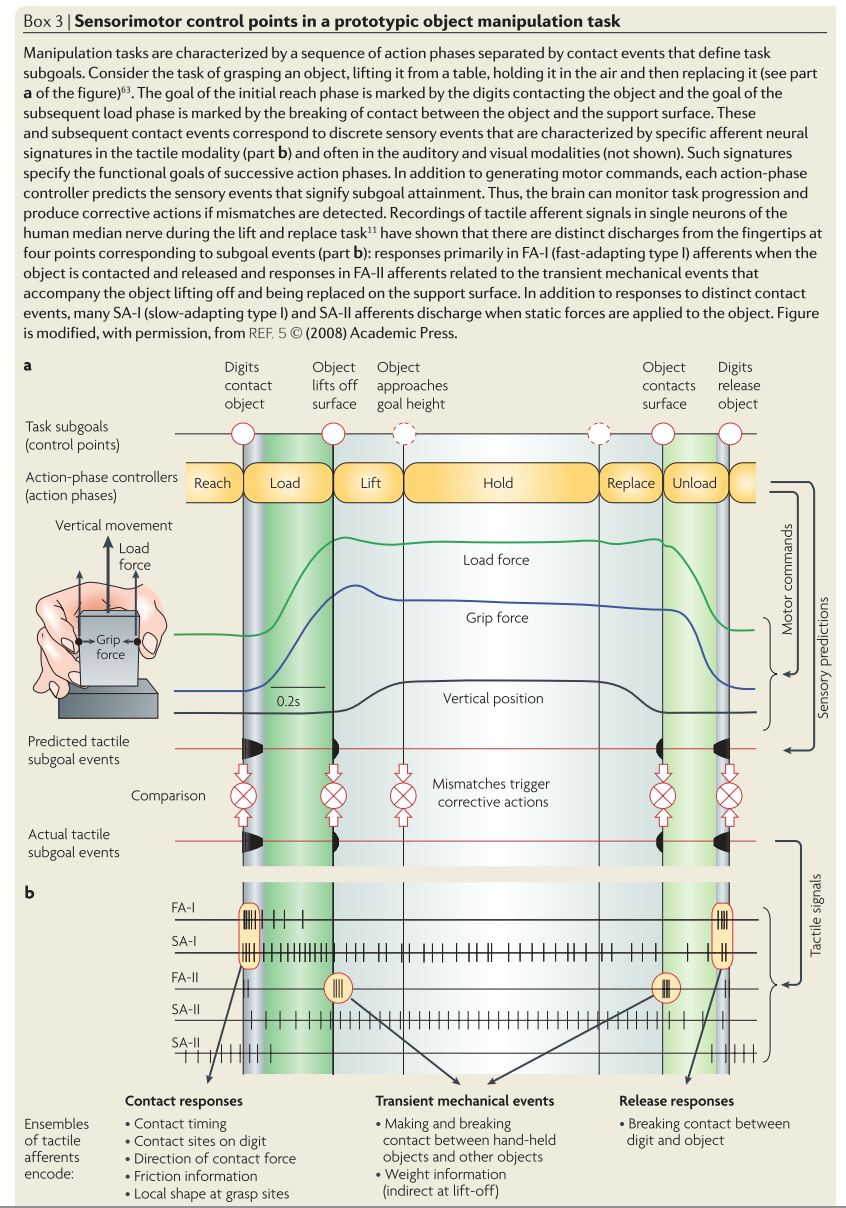
\includegraphics[width=12cm]{1_Bible/Photos/Biology/potentiel_daction.png}
	\caption{Exemple de séquence de potentiels d'action lors d'une tache de manipulation}\label{potentiel_daction}
\end{figure}


